%File: proposal.tex
\documentclass[letterpaper]{article} % DO NOT CHANGE THIS
\usepackage{aaai25}  % DO NOT CHANGE THIS
\usepackage{times}  % DO NOT CHANGE THIS
\usepackage{helvet}  % DO NOT CHANGE THIS
\usepackage{courier}  % DO NOT CHANGE THIS
\usepackage[hyphens]{url}  % DO NOT CHANGE THIS
\usepackage{graphicx} % DO NOT CHANGE THIS
\urlstyle{rm} % DO NOT CHANGE THIS
\def\UrlFont{\rm}  % DO NOT CHANGE THIS
\usepackage{natbib}  % DO NOT CHANGE THIS AND DO NOT ADD ANY OPTIONS TO IT
\usepackage{caption} % DO NOT CHANGE THIS AND DO NOT ADD ANY OPTIONS TO IT
\frenchspacing  % DO NOT CHANGE THIS
\setlength{\pdfpagewidth}{8.5in} % DO NOT CHANGE THIS
\setlength{\pdfpageheight}{11in} % DO NOT CHANGE THIS
%
% These are recommended to typeset algorithms but not required. See the subsubsection on algorithms. Remove them if you don't have algorithms in your paper.
\usepackage{algorithm}
\usepackage{algorithmic}

%
% These are are recommended to typeset listings but not required. See the subsubsection on listing. Remove this block if you don't have listings in your paper.
\usepackage{newfloat}
\usepackage{listings}
\DeclareCaptionStyle{ruled}{labelfont=normalfont,labelsep=colon,strut=off} % DO NOT CHANGE THIS
\lstset{%
	basicstyle={\footnotesize\ttfamily},% footnotesize acceptable for monospace
	numbers=left,numberstyle=\footnotesize,xleftmargin=2em,% show line numbers, remove this entire line if you don't want the numbers.
	aboveskip=0pt,belowskip=0pt,%
	showstringspaces=false,tabsize=2,breaklines=true}
\floatstyle{ruled}
\newfloat{listing}{tb}{lst}{}
\floatname{listing}{Listing}
%
% Keep the \pdfinfo as shown here. There's no need
% for you to add the /Title and /Author tags.
\pdfinfo{
/TemplateVersion (2025.1)
}

% DISALLOWED PACKAGES
% \usepackage{authblk} -- This package is specifically forbidden
% \usepackage{balance} -- This package is specifically forbidden
% \usepackage{color (if used in text)
% \usepackage{CJK} -- This package is specifically forbidden
% \usepackage{float} -- This package is specifically forbidden
% \usepackage{flushend} -- This package is specifically forbidden
% \usepackage{fontenc} -- This package is specifically forbidden
% \usepackage{fullpage} -- This package is specifically forbidden
% \usepackage{geometry} -- This package is specifically forbidden
% \usepackage{grffile} -- This package is specifically forbidden
% \usepackage{hyperref} -- This package is specifically forbidden
% \usepackage{navigator} -- This package is specifically forbidden
% (or any other package that embeds links such as navigator or hyperref)
% \indentfirst} -- This package is specifically forbidden
% \layout} -- This package is specifically forbidden
% \multicol} -- This package is specifically forbidden
% \nameref} -- This package is specifically forbidden
% \usepackage{savetrees} -- This package is specifically forbidden
% \usepackage{setspace} -- This package is specifically forbidden
% \usepackage{stfloats} -- This package is specifically forbidden
% \usepackage{tabu} -- This package is specifically forbidden
% \usepackage{titlesec} -- This package is specifically forbidden
% \usepackage{tocbibind} -- This package is specifically forbidden
% \usepackage{ulem} -- This package is specifically forbidden
% \usepackage{wrapfig} -- This package is specifically forbidden
% DISALLOWED COMMANDS
% \nocopyright -- Your paper will not be published if you use this command
% \addtolength -- This command may not be used
% \balance -- This command may not be used
% \baselinestretch -- Your paper will not be published if you use this command
% \clearpage -- No page breaks of any kind may be used for the final version of your paper
% \columnsep -- This command may not be used
% \newpage -- No page breaks of any kind may be used for the final version of your paper
% \pagebreak -- No page breaks of any kind may be used for the final version of your paperr
% \pagestyle -- This command may not be used
% \tiny -- This is not an acceptable font size.
% \vspace{- -- No negative value may be used in proximity of a caption, figure, table, section, subsection, subsubsection, or reference
% \vskip{- -- No negative value may be used to alter spacing above or below a caption, figure, table, section, subsection, subsubsection, or reference

\setcounter{secnumdepth}{2} %May be changed to 1 or 2 if section numbers are desired.

% The file aaai25.sty is the style file for AAAI Press
% proceedings, working notes, and technical reports.
%

\usepackage{amsmath}
\usepackage{hyperref}
\hypersetup{
    colorlinks = true,
    allcolors = blue
}

% Title

% Your title must be in mixed case, not sentence case.
% That means all verbs (including short verbs like be, is, using, and go),
% nouns, adverbs, adjectives should be capitalized, including both words in hyphenated terms, while
% articles, conjunctions, and prepositions are lower case unless they
% directly follow a colon or long dash
\title{CS 598 Deep Learning for Healthcare\\Project Proposal}
\author {Eric Schrock}
\affiliations{ejs9@illinois.edu}

\begin{document}

\maketitle

\section{Introduction}

\subsection{Proposed Project}

For my project, I propose to reproduce some or all of the findings of the paper, "Multi-Label Generalized Zero Shot Learning for the Classification of Disease in Chest Radiographs" \cite{hayat2021multilabel}. Compute power will likely determine whether I am able to reproduce the full set of findings or merely a subset, given the time remaining in the semester (more about this in Section~\ref{sec:computation-feasibility}). In addition to reproducing original findings, I propose to implement and test at least one ablation or extension of the work done by the authors of the paper (see Section~\ref{sec:ablations-and-extensions}).

\subsection{Problem Statement}

Deep learning models for classifying diseases from chest X-ray (CXR) images have had great success, achieving comparable results to human experts. However, collecting and labeling training data for these models is expensive and time-consuming. For rarer diseases, it is often not economical, and sometimes not even possible, to gather the amount of data needed for supervised learning models. When a new disease emerges, the need for massive data collection slows the response. Human radiologists leverage other sources of knowledge to identify diseases they have previously never seen in X-ray form. Could a deep learning model do the same?

Multi-label generalized zero shot learning (ML-GZSL), which uses semantic information to identify classes not present in the set of labeled images used to train the model, has worked well in similar circumstances \cite{10.1109/TPAMI.2012.256, 10.1109/TMM.2019.2924511, 9157745}. However, these prior works have at least two limitations. First, they "extract a fixed visual representation of the image from a pre-trained visual encoder or a detection network" \cite{hayat2021multilabel}, which means they cannot be trained end-to-end. Second, "projecting these extracted visual features to the semantic space shrinks the diversity of the visual information, which gives rise to inherent limitations" \cite{hayat2021multilabel}, one of those being the hubness problem \cite{dinu2015improvingzeroshotlearningmitigating}. Can these limitations be overcome?

\section{Methodology}

\subsection{Specific Approach}

The paper in question proposes the CXR-ML-GZSL model, shown in Figure~\ref{fig:model}. It is comprised of a pre-trained text encoder to convert class labels to a semantic embedding space, a trainable visual encoder to convert X-ray images to a visual embedding space, and mapping models into a shared latent embedding space. The output is a score for each possible class, representing how relevant it is to the input image.

\begin{figure}[h!]
\centering
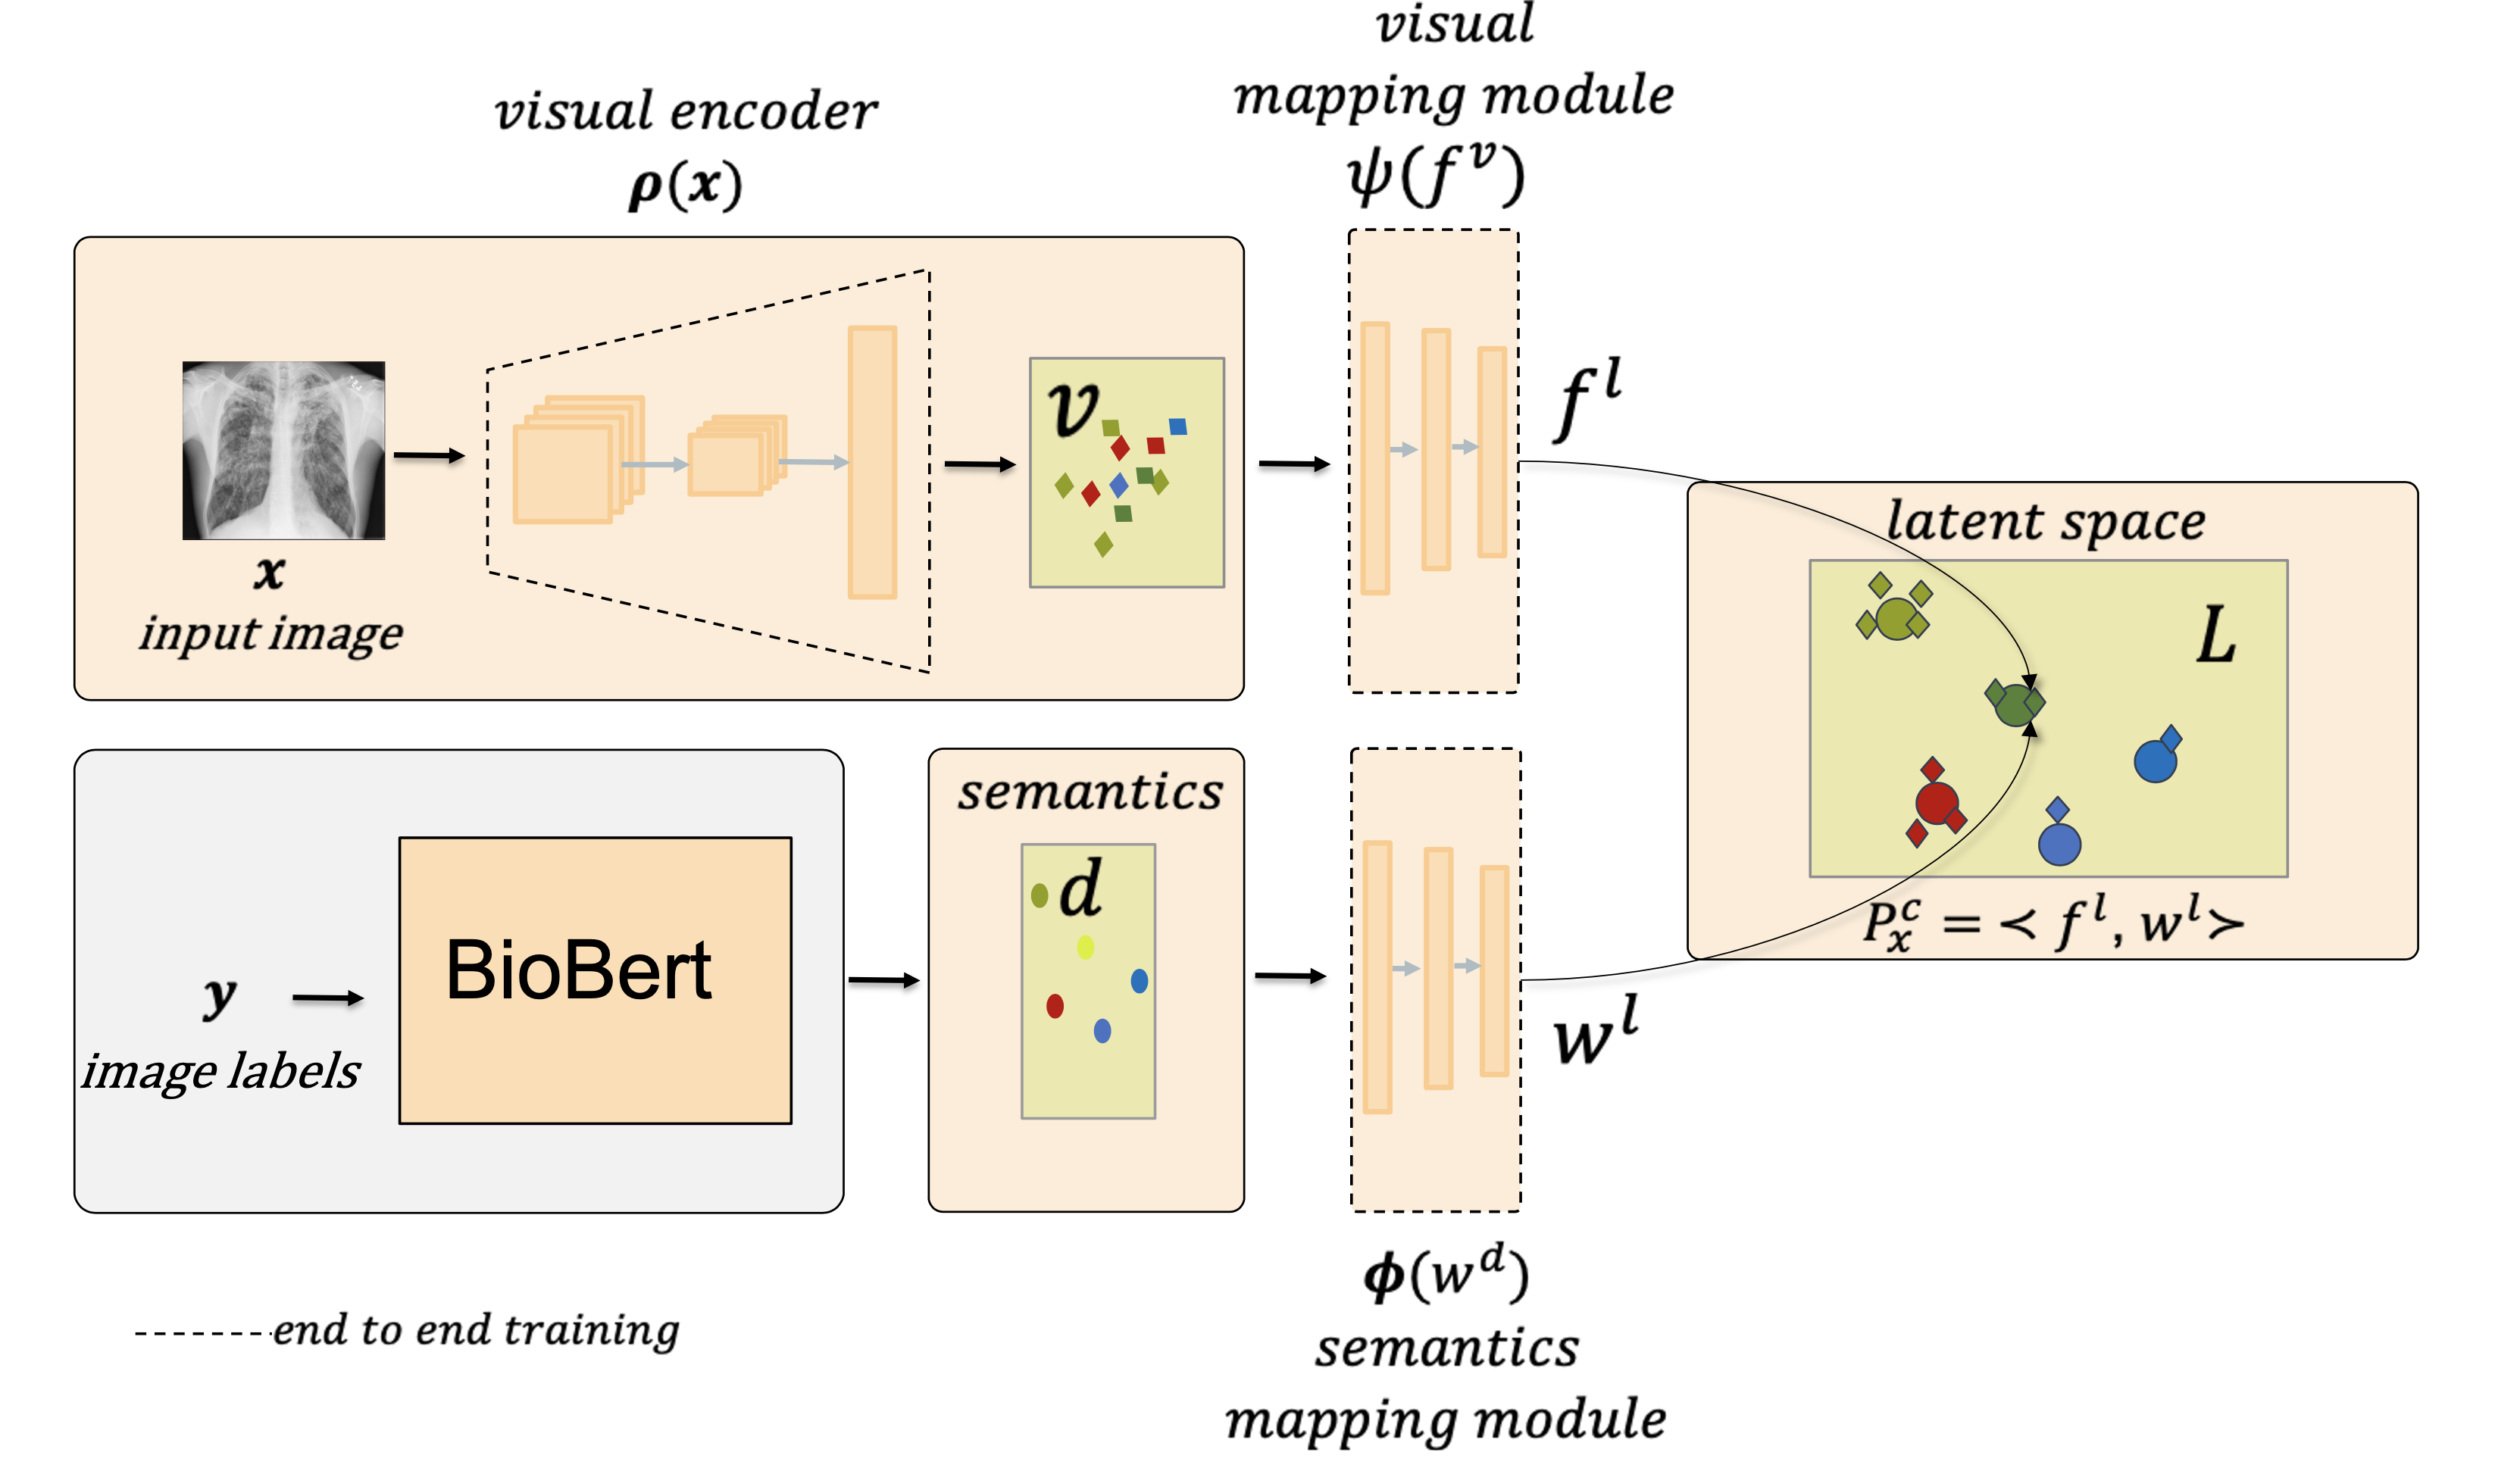
\includegraphics[width=0.9\columnwidth]{model.png}
\caption{CXR-ML-GZSL \cite{hayat2021multilabel}}
\label{fig:model}
\end{figure}

Since the visual encoder is trainable, the whole pipeline between the X-ray image and the semantic embedding of the class label is trainable from end-to-end, better tuning the overall model to the task at hand. Additionally, the added latent embedding space is meant to address the limitations of mapping the visual embedding space directly onto the semantic embedding space.

The increased complexity of this model, compared to other ML-GZSL models, requires a multifaceted training objective, captured in a three-part loss function, where $\gamma_1$ and $\gamma_2$ are the regularization parameters for the second and third components of the loss function.

\begin{equation}
    \min_{\boldsymbol{\phi} ,\boldsymbol{\rho} ,\boldsymbol{\psi}} \mathcal{L} = \mathcal{L}_{{rank}} +\gamma_{1} \mathcal{L}_{align} +\gamma_{2} \mathcal{L}_{con},
    \label{eqn:full_loss}
\end{equation}

\texorpdfstring{$\mathcal{L}_{rank}$}: adds penalties for any positive ground-truth relevance scores not larger than all negative grouth-truth relevance scores by at least a margin of $\delta$. \texorpdfstring{$\mathcal{L}_{align}$}: adds penalties if input images and their labels do not map near each other in the latent embedding space. \texorpdfstring{$\mathcal{L}_{con}$}: add penalties if labels do not have similar relationships in both the semantic and latent embedding spaces, as those semantic relationships are key to zero shot learning. 

For the pre-trained text encoder, the model uses BioBERT \cite{10.1093/bioinformatics/btz682}, which was trained specifically on a biomedical corpora. For the trainable visual encoder, the model uses Densenet-121 \cite{rajpurkar2017chexnetradiologistlevelpneumoniadetection}, as at that time it was the best chest X-ray classifier. For both BioBERT and Densenet-121, the model skips the final classification step in order to get semantic and visual embeddings, respectively, as output instead. The two mapping models are both three layer feed-forward neural networks.

The model was trained over 100 epochs using the Adam optimizer \cite{kingma2017adammethodstochasticoptimization}, with multiple repetitions to tune the learning rate, $\gamma_1$, and $\gamma_2$ hyperparameters. It's performance was measured using the "overall precision, recall and f1 scores for the top $k$ predictions where $k \in \{2, 3 \}$ [as well as] the average area under the receiving operating characteristic curve (AUROC) for seen and unseen classes and its harmonic mean, since computing recall for top k predictions may not be a sufficient indicator of class-wise performance" \cite{hayat2021multilabel}.

\subsection{Novelty, Relevance, and Hypotheses}

CXR-ML-GZSL is the first use of ML-GZSL to classify diseases from chest X-ray images. It is also unique from other ML-GZSL models in the following three ways.

\begin{itemize}
    \item It can be trained end-to-end, thanks to the trainable visual encoder.
    \item It maps both the semantic and visual embedding spaces into a shared latent embedding space, instead of mapping the visual space onto the semantic space, loosing less visual information.
    \item It uses BioBERT, which is trained on a biomedical corpora, resulting semantic embeddings that are tuned for healthcare use cases.
\end{itemize}

The hypothesis is that these improvements will result in better performance when classifying both seen and unseen diseases in chest X-ray images, compared to two state-of-the-art ML-GZSL models: LESA \cite{9157745} and MLZSL \cite{lee2018multilabelzeroshotlearningstructured}. The results in Figure~\ref{fig:results} bear this out.

\begin{figure}[h!]
\centering
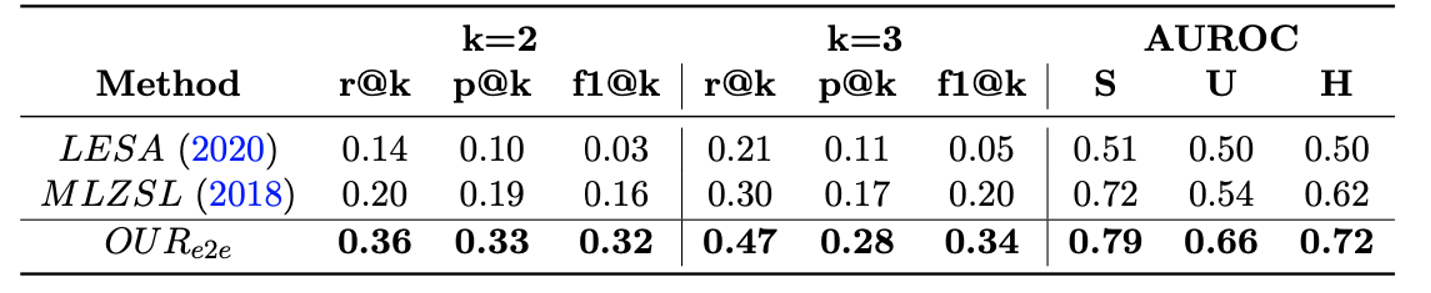
\includegraphics[width=0.9\columnwidth]{results.png}
\caption{Performance of LESA, MLZSL, and CXR-ML-ZSL (``$OUR_{e2e}$") on the ChestX-ray8 database \cite{Wang_2017}. Metrics are precision, recall, f1, and AUROC (split by seen, unseen, and the harmonic mean of the two) \cite{hayat2021multilabel}.}
\label{fig:results}
\end{figure}

\subsection{Ablations and Extensions}
\label{sec:ablations-and-extensions}

TBD

\section{Data Access and Implementation Details}

\subsection{Dataset}

TBD

\subsection{Model and Codebase}

TBD

\subsection{Computation Feasibility}
\label{sec:computation-feasibility}

TBD

\bibliography{proposal}

\end{document}
